%%%%%%%%%%%%%%%%%%%%%%%%%%%%%%%%%%%%%
%% Supporting Information
%% (Optional)
%%%%%%%%%%%%%%%%%%%%%%%%%%%%%%%%%%%%%
% OVERVIEW
%
% Please note that all supporting information will be peer reviewed with your manuscript.
% In general, the purpose of the supporting information is to enable
% authors to provide and archive auxiliary information such as data
% tables, method information, figures, video, or computer software,
% in digital formats so that other scientists can use it.

% The key criteria are that the data:
% 1. supplement the main scientific conclusions of the paper but are not essential to the conclusions (with the exception of
%    including data so the experiment can be reproducible);
% 2. are likely to be usable or used by other scientists working in the field;
% 3. are described with sufficient precision that other scientists can understand them, and
% 4. are not exe files.
%

% All Supporting text and figures should be included in this document.

% Data sets, large tables, movie files,
% and audio files should be uploaded separately, following AGU naming
% conventions. Include their captions in this document and list the
% file name with the caption. You will be prompted to upload these
% files on the Upload Files tab during the submission process, using
% file type “Supporting Information (SI)”

\documentclass[draft]{agujournal}
\graphicspath{{figures/}}

\usepackage{amsmath}
\usepackage{apacite}
%\usepackage[font=normalsize]{caption}
% \bibliographystyle{agu08}
% \setcitestyle{authoryear,open={[},close={]}}

\renewcommand{\figurename}{Figure S}
\renewcommand{\tablename}{Table S}

% Please type in the journal name: \journalname{<Journal Name>}
% ie,
\journalname{Journal of Geophysical Research}

%% Choose from this list of Journals:
%
% Journal of Geophysical Research
% JGR-Biogeosciences
% JGR-Earth Surface
% JGR-Planets
% JGR-Solid Earth
% JGR-Space Physics
% Global Biochemical Cycles
% Geophysical Research Letters
% Paleoceanography
% Radio Science
% Reviews of Geophysics
% Tectonics
% Space Weather
% Water Resource Research
% Geochemistry, Geophysics, Geosystems
% Journal of Advances in Modeling Earth Systems (JAMES)
% Earth's Future
% Earth and Space Science

\begin{document}

%% This command needs article title as argument to \supportinginfo{}:
\supportinginfo{What controls variations in aftershock productivity?}

\authors{Kelian Dascher-Cousineau \affil{1},
 Emily E. Brodsky \affil{1}, Thorne Lay \affil{1}
 }
 
\affiliation{1}{University of California Santa Cruz, Santa Cruz, California, USA.} 



%% ------------------------------------------------------------------------ %%
%
%  TEXT
%
%% ------------------------------------------------------------------------ %%

\section*{Contents}
%%%Remove or add items as needed%%%
\begin{enumerate}
\item Sensitivity to magnitude of completeness
\item Relative productivity as a function of miscellaneous parameters
\item Catalogued source attributes
\item Figures S1 to S12
\end{enumerate}

\section*{Sensitivity to magnitude of completeness}
We test the robustness of our significant findings by testing their validity with a magnitude of completeness of $M_w5$ instead of $M_w4.5$ as done in the main text. Figures are ordered as presented in the text.

%%%%%%%%%%%%%%%%%%%%%%%%%%%%%%%%%%%%%%%%%%%%%%%%%%%%%%%%%%%%%%%%%%%%%%%%
\begin{figure}[!ht]
\centering
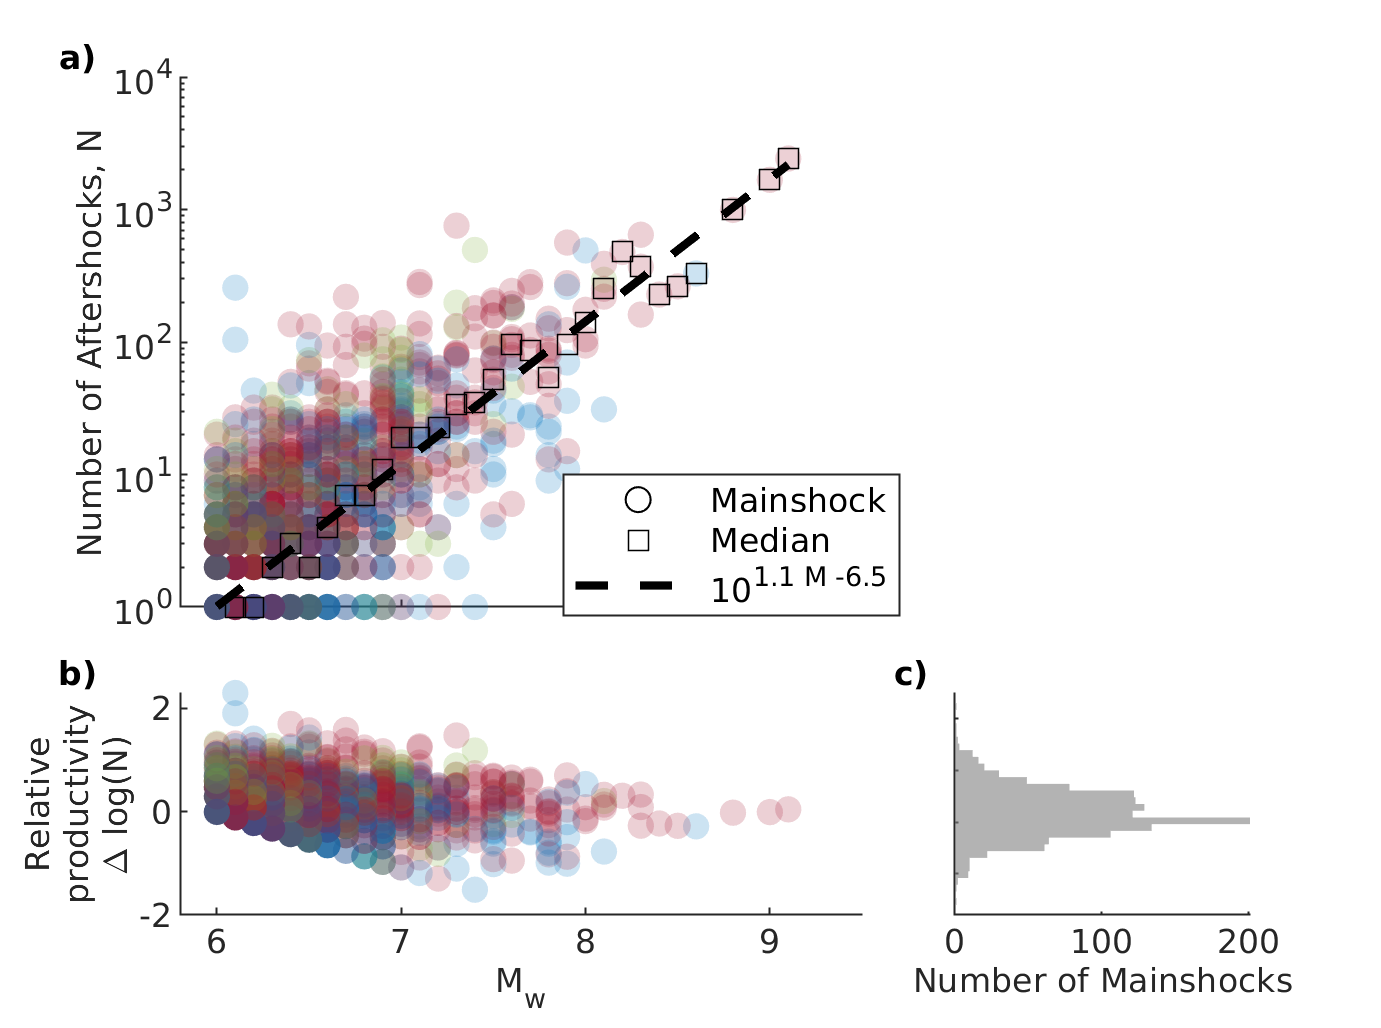
\includegraphics{figures/prod_law_mw5.png}
\caption{The number of aftershocks of $M_W\ge5$ within three source dimensions and 60 days as a function of mainshock magnitude identified in the global ISC and NEIC catalogs from 1990 to 2019. Colors indicate faulting style of the mainshock; blue, green and red points correspond to earthquake sequences for which the mainshock was respectively strike-slip, normal or reverse. The global productivity law (dashed line) is fit using a least squares regression through the median log-number of aftershocks for each 0.1 magnitude bin (black squares). The median number includes mainshocks with no aftershocks which are not shown on the plot. Note the individual earthquake sequences (circles) exhibit significant scatter around the productivity law. b) Relative productivity as a function of mainshock magnitude. The relative productivity distribution does not show events with no aftershocks and thus the lower left corner of the plot is underpopulated. c) Histogram of the relative productivity of mainshocks considered in this study.
}
\label{fig:fms_prod}
\end{figure}

\begin{sidewaysfigure}
\centering
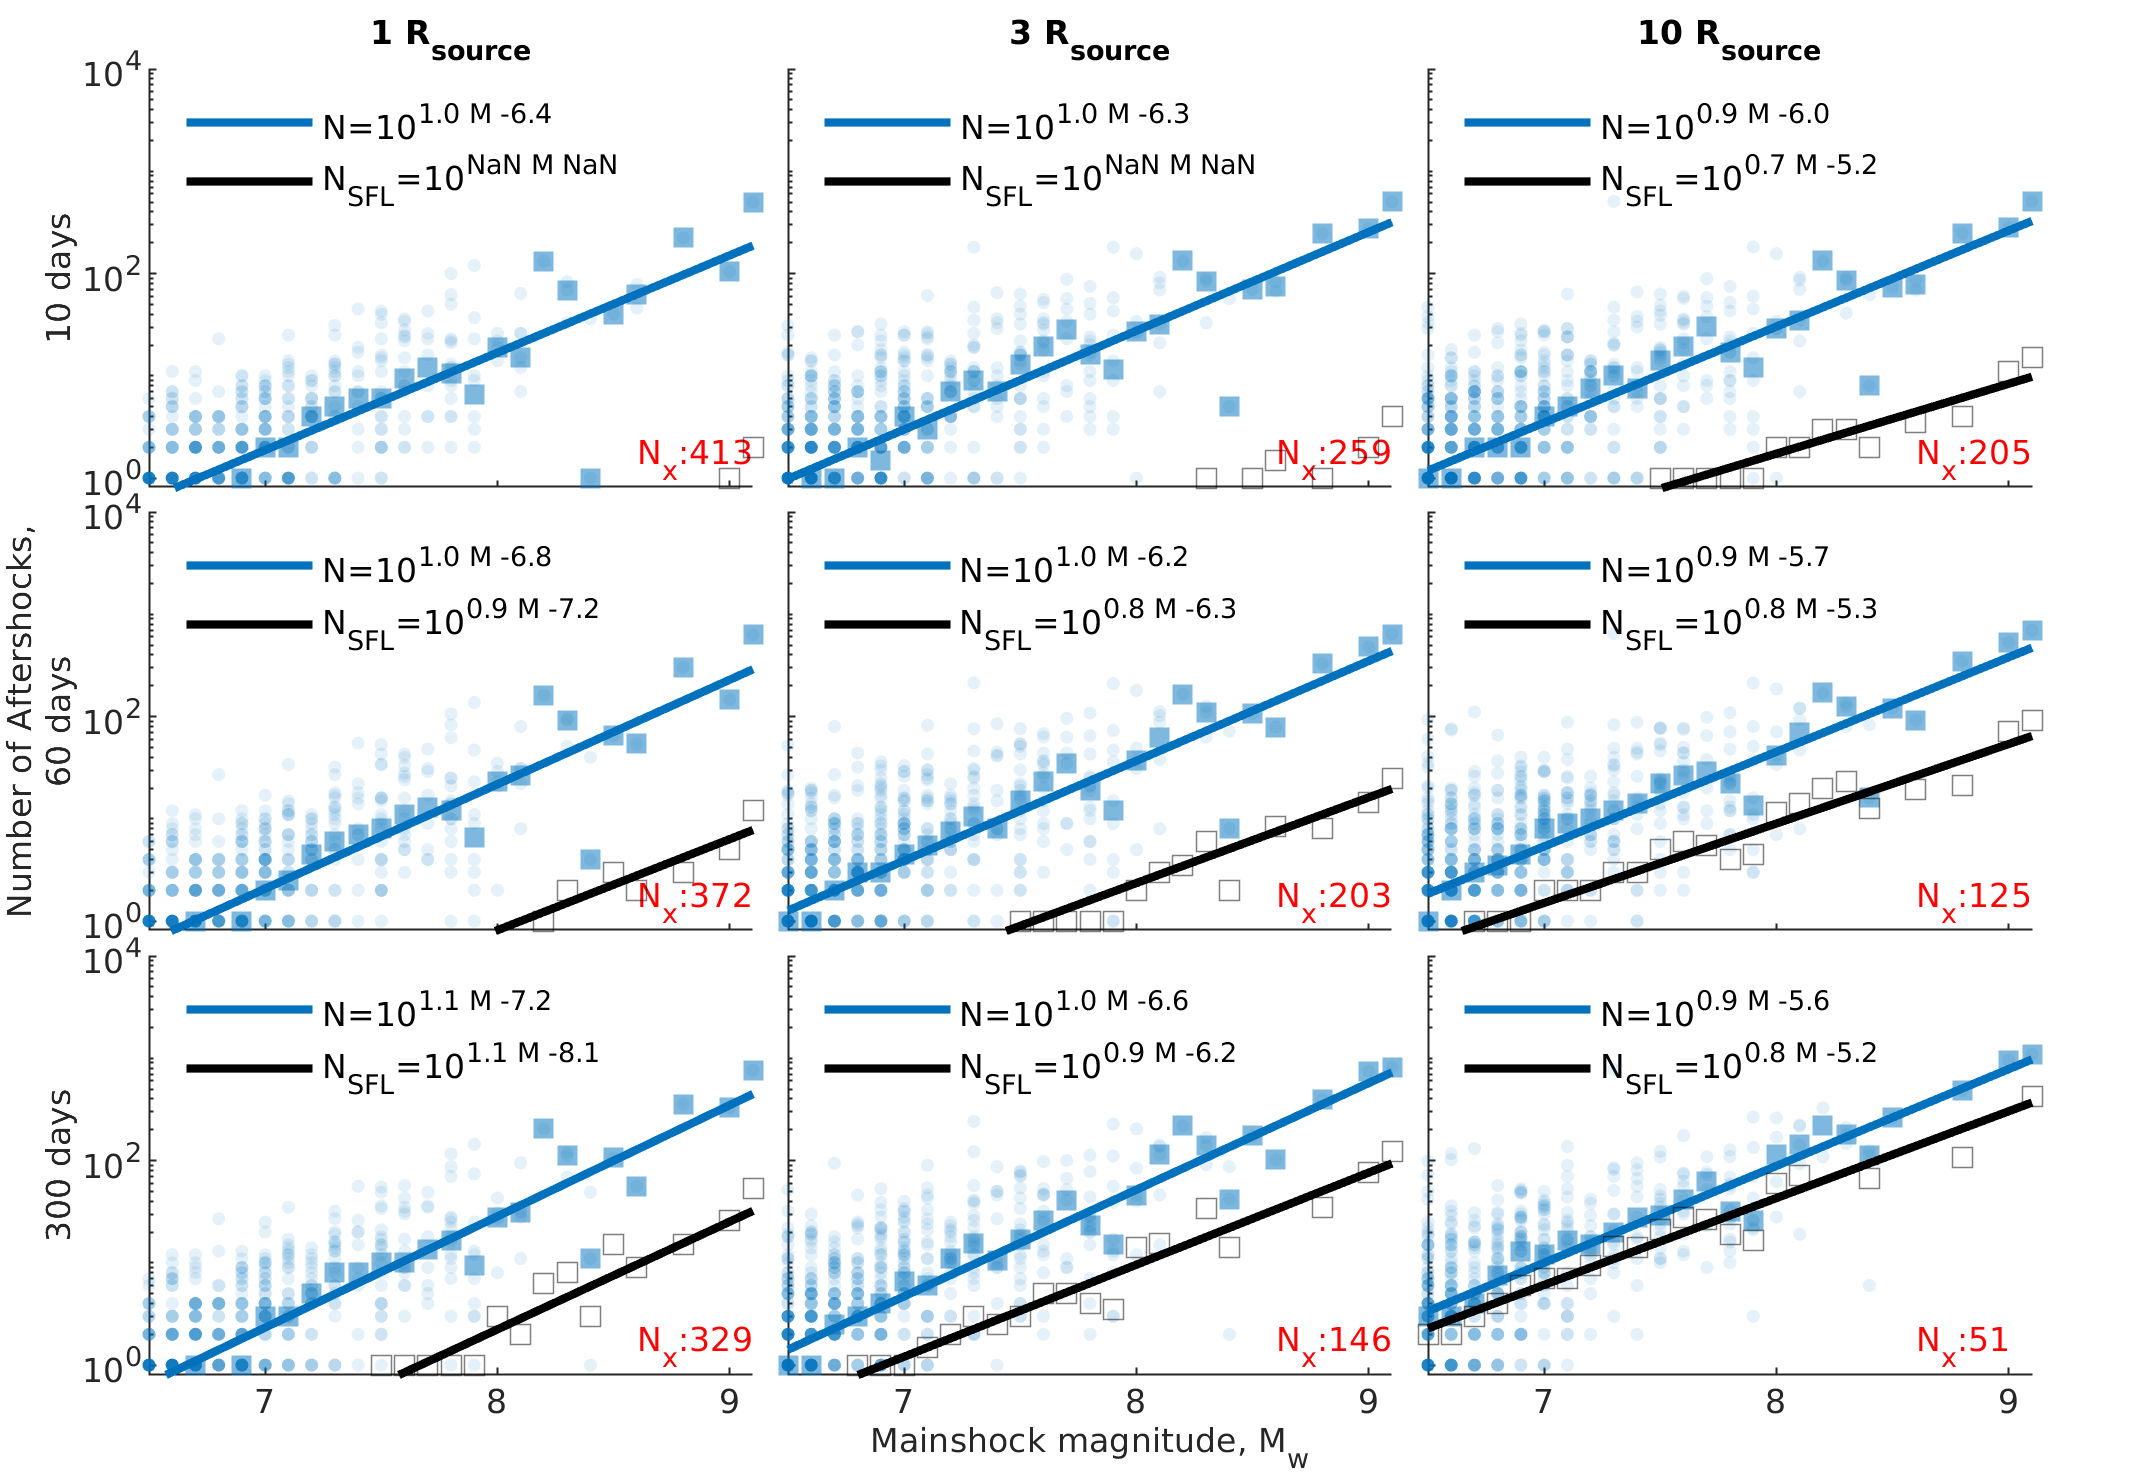
\includegraphics{figures/sensitivity_mw5.png}
\caption{Sensitivity analysis of space-time windows for $M_W$>5. Time windows of 10, 60, and 100 days and spherical space with radii of 1, 3, and 10 source dimensions ($R_{source}$) are considered. Blue data are mainshocks identified through our hierarchical declustering routine. Circles are individual mainshocks. Squares are median values for each 0.1 magnitude bins. Regressions are computed using least squares through the median log-number of aftershocks for each 0.1 magnitude bin. For reference, we computed the median productivity relationship (grey squares) for 100 time-shuffled catalogs and the corresponding scaling relationship (black line). For each space-time window, we indicate the number of mainshocks with no aftershocks in red ($N_x$). Note that as space and time windows increase, more mainshocks have measurable aftershock counts. However, the likelihood of counting background productivity and significantly affecting subsequent parameterization becomes an increasing concern.}
\label{fig:sensitivity}
\end{sidewaysfigure} 

\begin{sidewaysfigure}
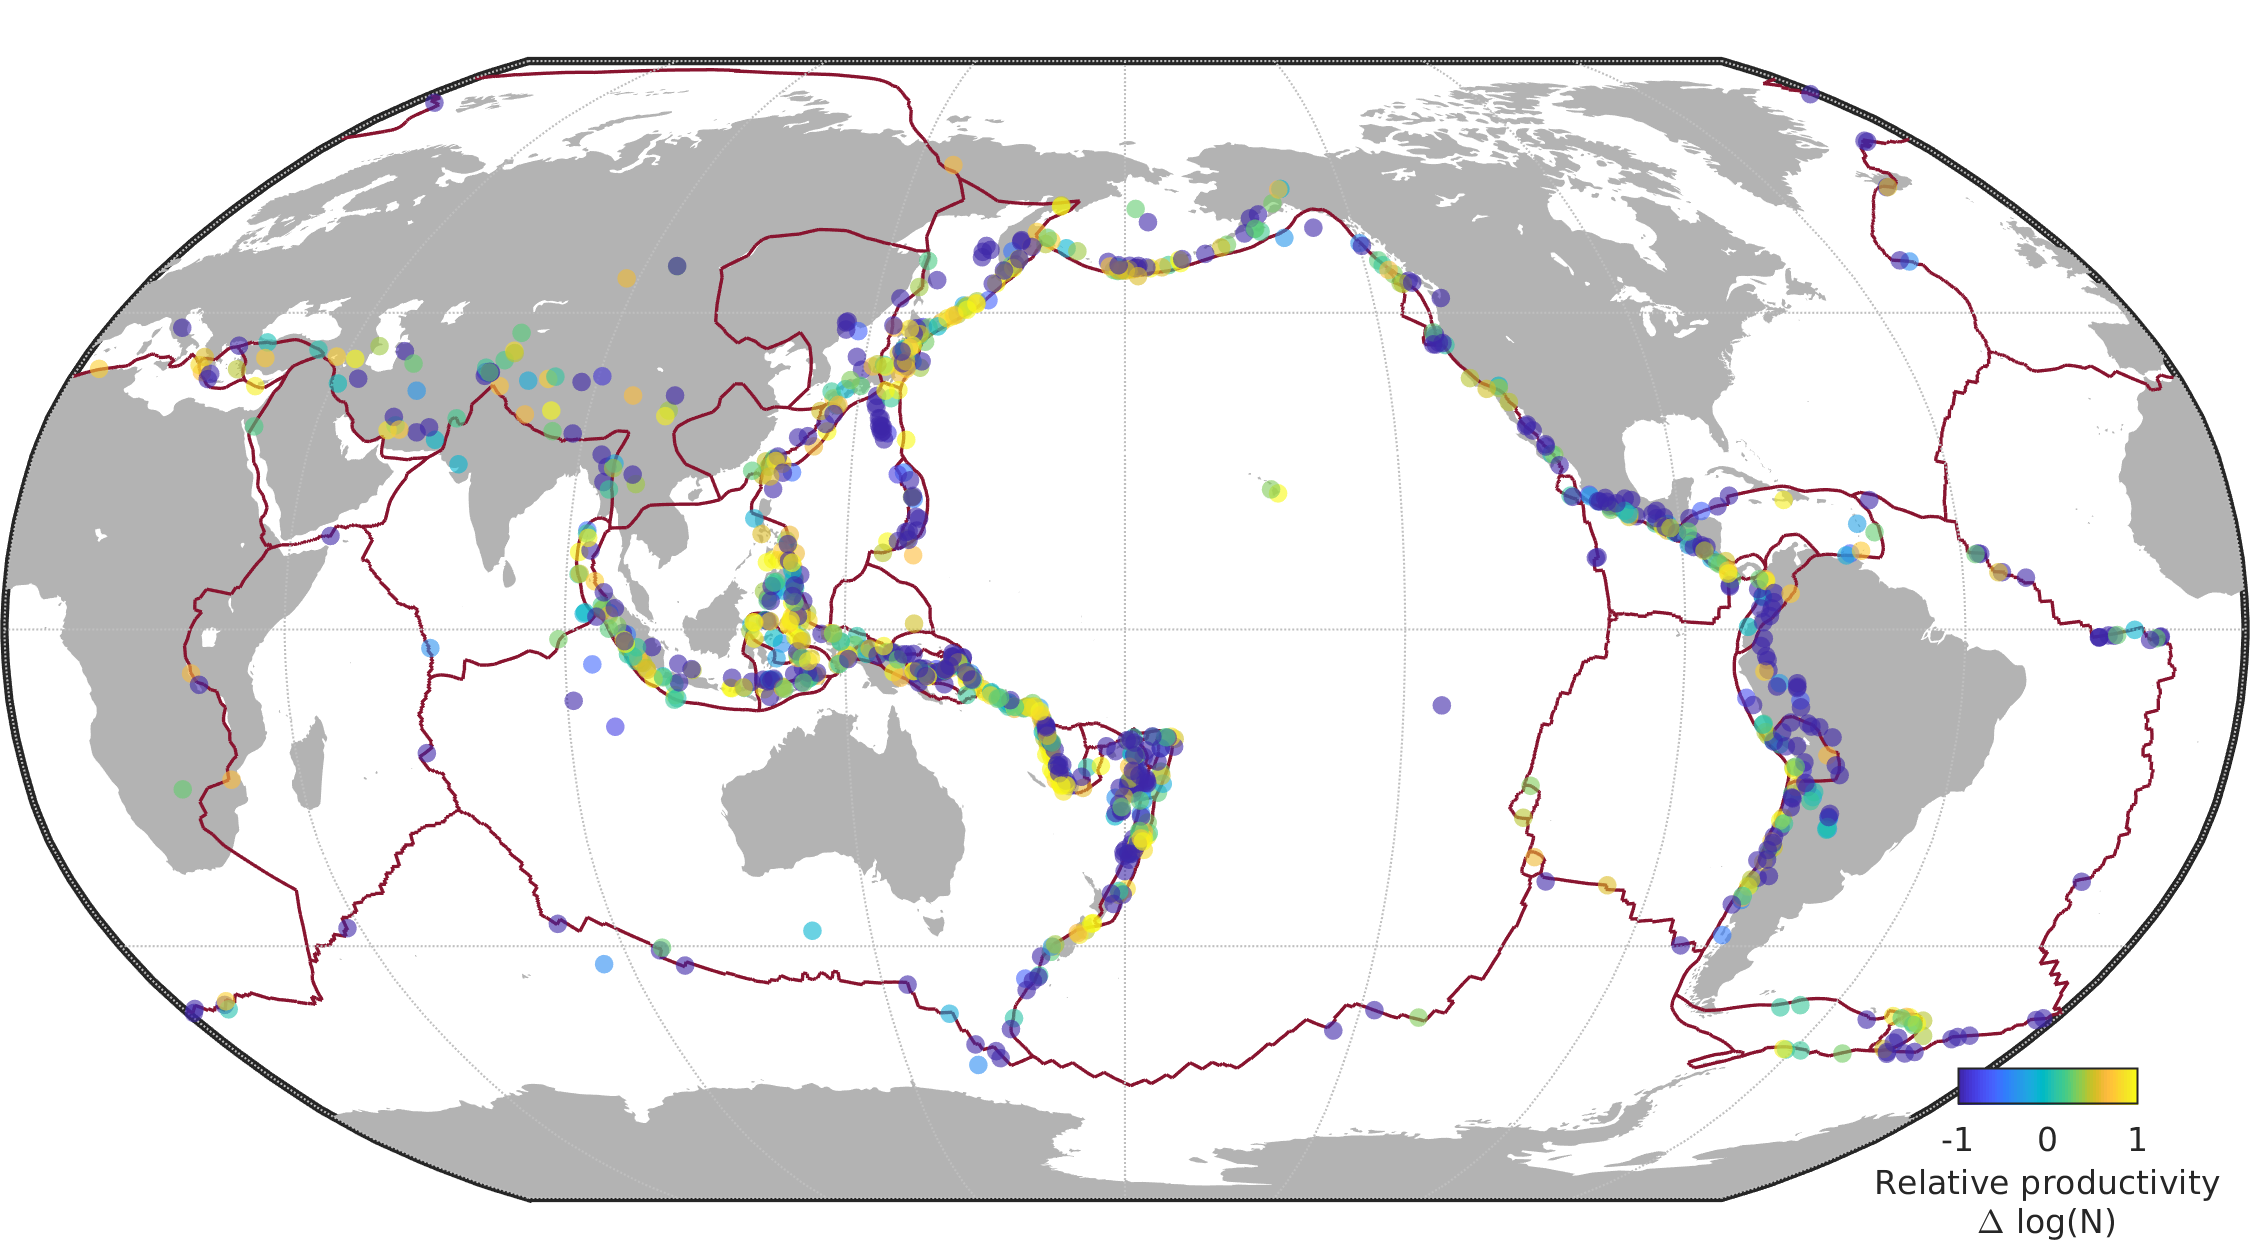
\includegraphics{figures/worldmap_res_mw5.png}
\caption{Global map of earthquake productivity for $M_W$>5. Red lines indicate the surface trace of the tectonic boundaries. Mainshocks with $M_W\ge6.5$ color-coded according to their relative productivity.)
} 
\label{fig:global_res}
\end{sidewaysfigure}

\begin{figure}
\centering
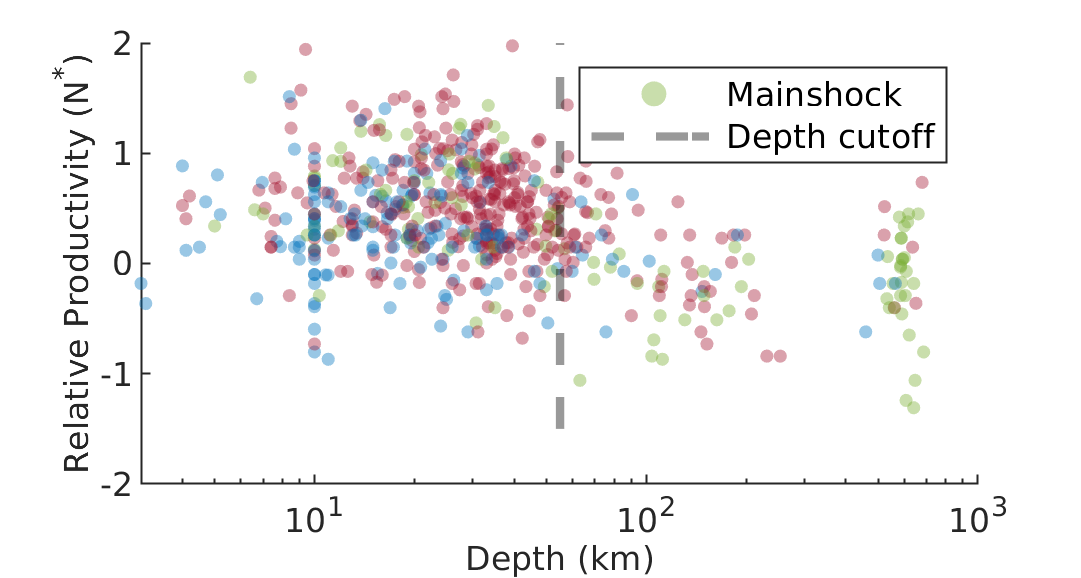
\includegraphics{figures/prod_vs_depth_mw5.png}
\caption{Relative aftershock productivity as a function of depth for $M_W$>5. Subsequent analysis will only consider earthquakes shallower than the 55 km cutoff (dashed line). Sequences are color-coded according to faulting style of the mainshock (blue: strike-slip, green: normal and red: reverse).}
\label{fig:prod_vs_depth}
\end{figure}


\begin{figure}
\centering
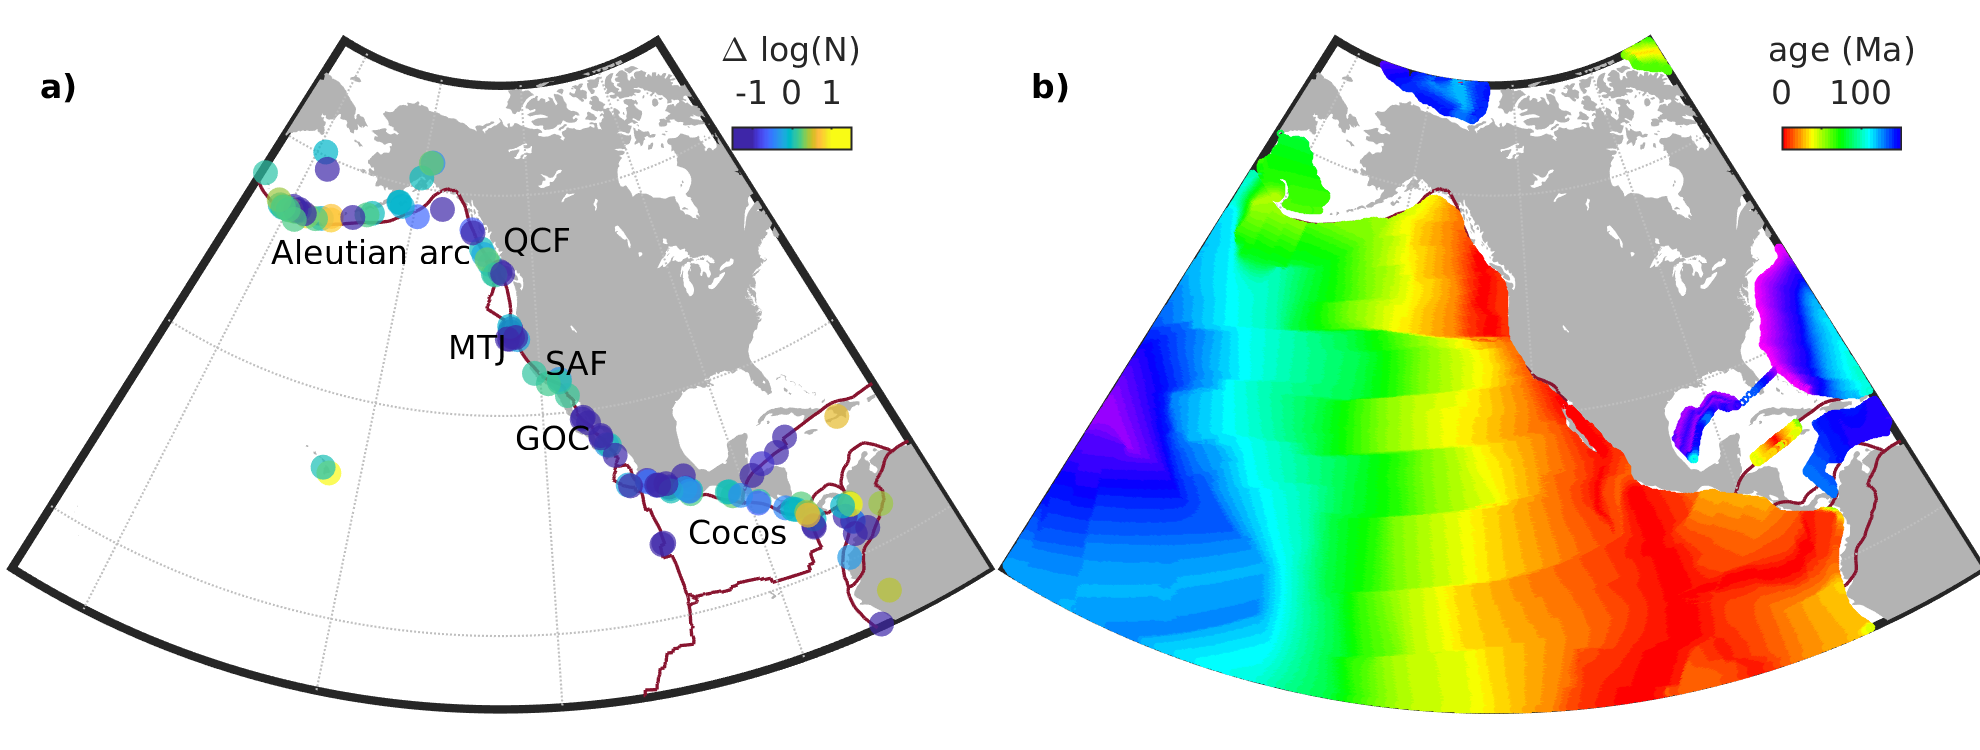
\includegraphics[]{figures/regions_mw5.png}
\caption{a) Aftershock productivity along the North American coastline for $M_W$>5.  Individual mainshocks (points) are color-coded according to their relative aftershock productivity ($\Delta \log(N)$). The Aleutian arc, the Queen Charlotte Fault (QCF), the Mendocino Triple Junction (MTJ), San Andreas Fault (SAF), the Gulf of California (GOC) and the Cocos plate subduction include areas with coherent productivity. Red line indicates major plate boundaries \citep{Bird2003AnBoundaries}. b) Seafloor crustal age estimates from \citet{Muller2008}.}
\label{fig:region}
\end{figure}  

\begin{figure}
\centering
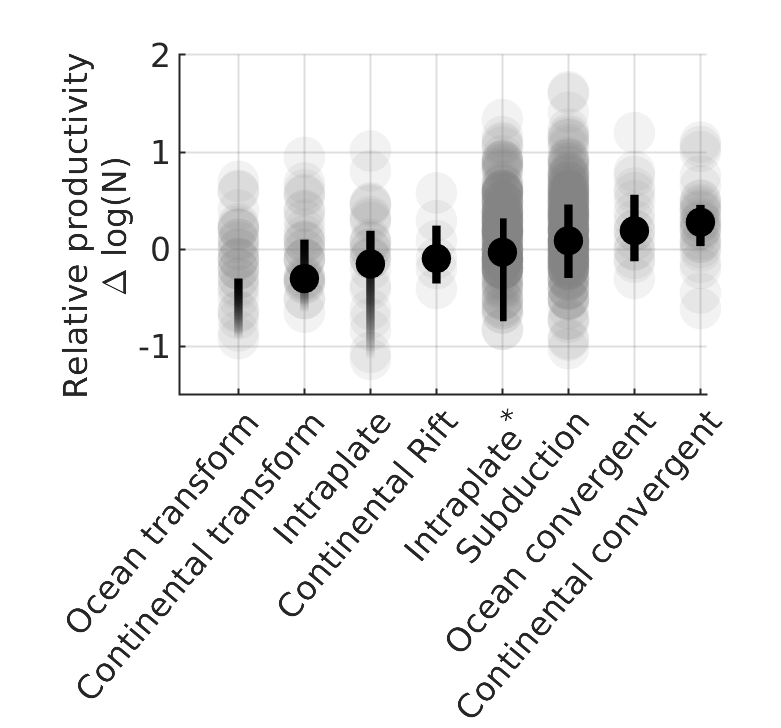
\includegraphics{figures/prod_by_pb_mw5.png}
\caption{Earthquake productivity by tectonic boundary for $M_W$>5. Points indicate the relative productivity of individual sequences. Solid markers and error bars indicate the median and the interquartile range. A faded lower error bar implies that mainshocks with no aftershocks are within the interquartile range. Intaplate$^*$ indicates earthquakes within 400km from a plate boundary but with a faulting mechanism discordant with the plate boundary (e.g., outer rise events).}
\label{fig:plate_boundary}
\end{figure}    


\begin{figure}
\centering
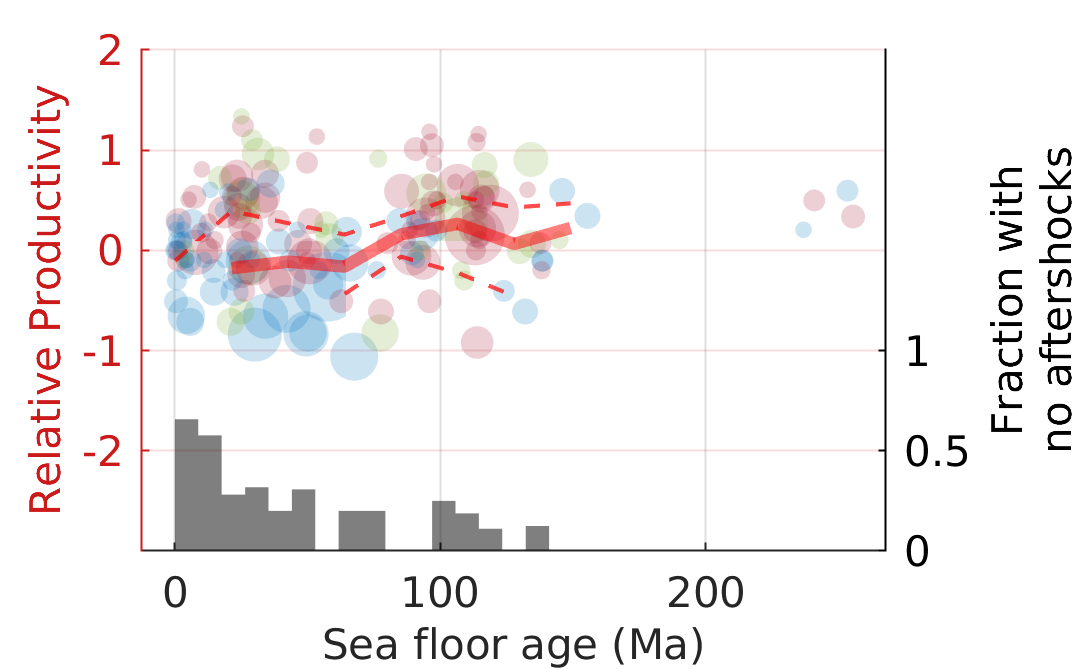
\includegraphics{figures/prod_vs_age_mw5.png}
\caption{Relative productivity increases as a function of the age of the oceanic lithosphere for $M_W$>5. Each point indicates an individual earthquake sequence. Sequences are color-coded by faulting style of the mainshock (blue: strike-slip, green: normal and red: reverse). The red line indicates the median average for 20Ma crustal age bins. Dashed lines indicate the corresponding interquartile ranges. Bars indicate the fraction of earthquakes with no aftershocks within each 10Ma crustal age bin.}
\label{fig:prod_vs_age}
\end{figure}   

\begin{figure}
\centering
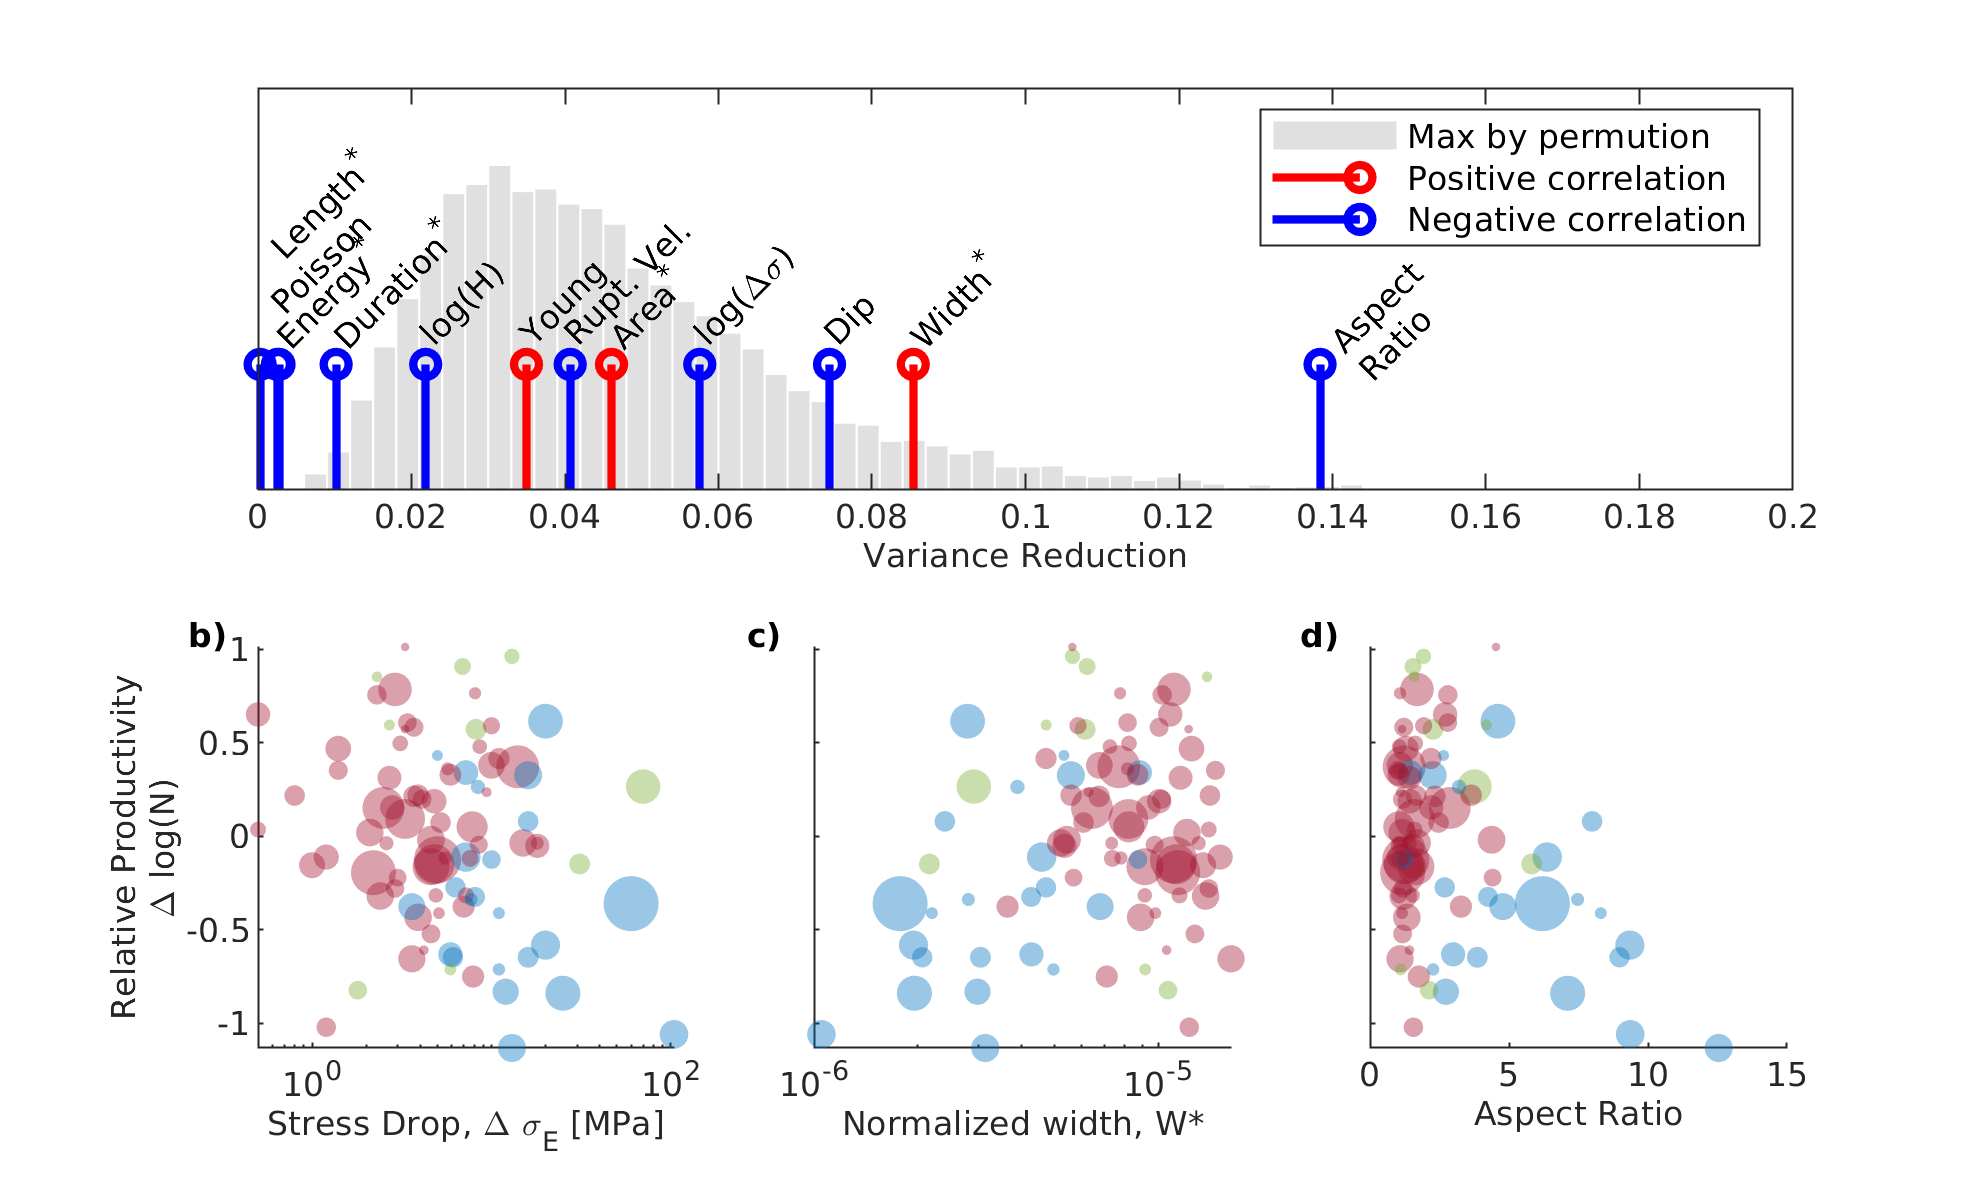
\includegraphics{figures/stem_plot_mw5.png}
\caption{a) Goodness of fit of linear regressions for each source attribute in our combined catalog for $M_W$>5. Top and bottom axes respectively represent the p-value and goodness of fit of each attribute (stems). The probability distribution function in the backdrop indicates the maximal variance reduction outcome of 10000 permutation test of the entire data set we tested. The probability of obtaining a spurious correlation by chance over the whole family of attributes we tested for is derived from the number of random shuffles exceeding the measured variance reduction and normalized to the overall sample (10000). Asterisks indicate scaled and log-transformed variables. The scaled energy, length, duration and area, material properties, velocity, dip, and stress drop ($\Delta\sigma$) of the mainshock rupture all do not yield a statistically significant ($p=0.05$) linear fit to the relative productivity — the normalized rupture width and aspect ratio of the rupture yield the best fitting linear regressions. Stems are color-coded to indicate whether the source attribute is positively (red) or negatively (blue) correlated with relative productivity. b-d): Relative earthquake productivity as a function of mainshock stress drop, normalized rupture width, and aspect ratio. Individual mainshocks are color-coded according to faulting style as in Figure \ref{fig:fms_prod}.}
\label{fig:r2_finite_fault}
\end{figure}

\begin{figure}
\centering
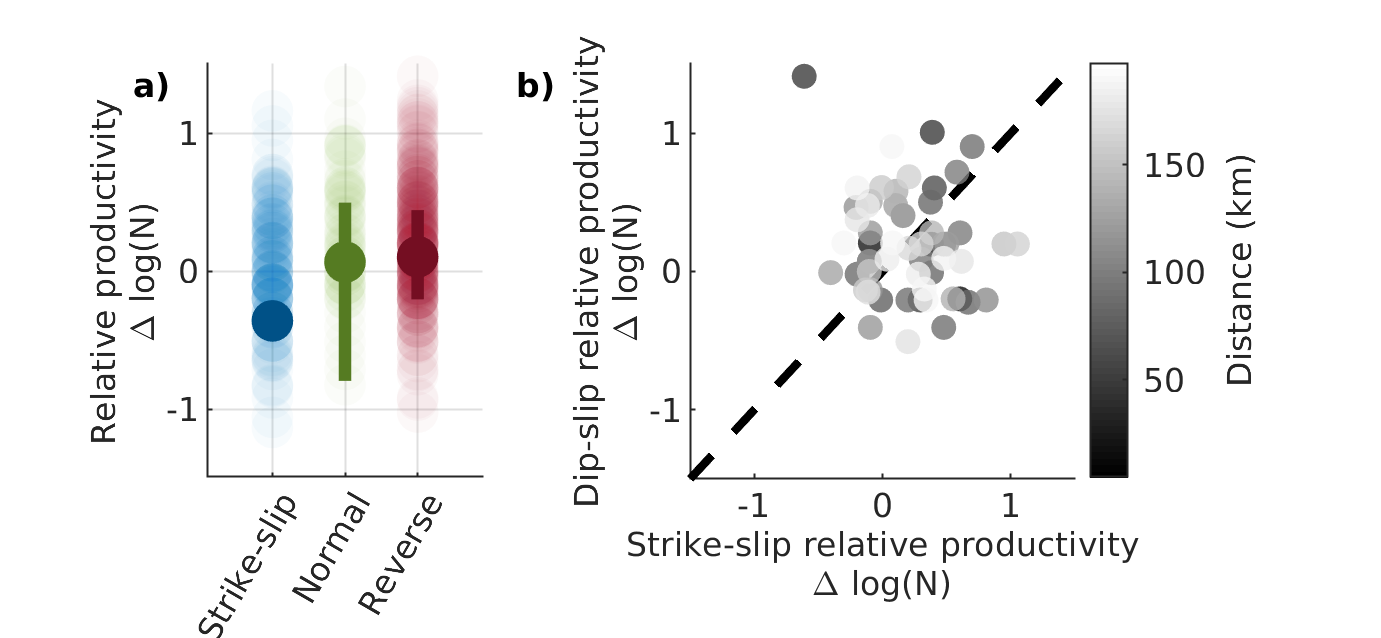
\includegraphics{figures/fmspairs_mw5.png}
\caption{a) Relative aftershock productivity  ($\Delta \log(N)$) for $M_W$>5 by focal mechanism. b) Relative aftershock productivity for pairs of earthquake sequences with strike-slip and dip-slip mainshocks within 200 km from each other. Each pair is shaded according to its relative distance. Dashed line indicates a 1:1 relationship, the expectation for a purely site dominated control on relative productivity. Co-located mainshocks pairs generally follow this 1:1 trend, but exhibit considerable scatter.}
\end{figure}

\begin{figure}
\centering
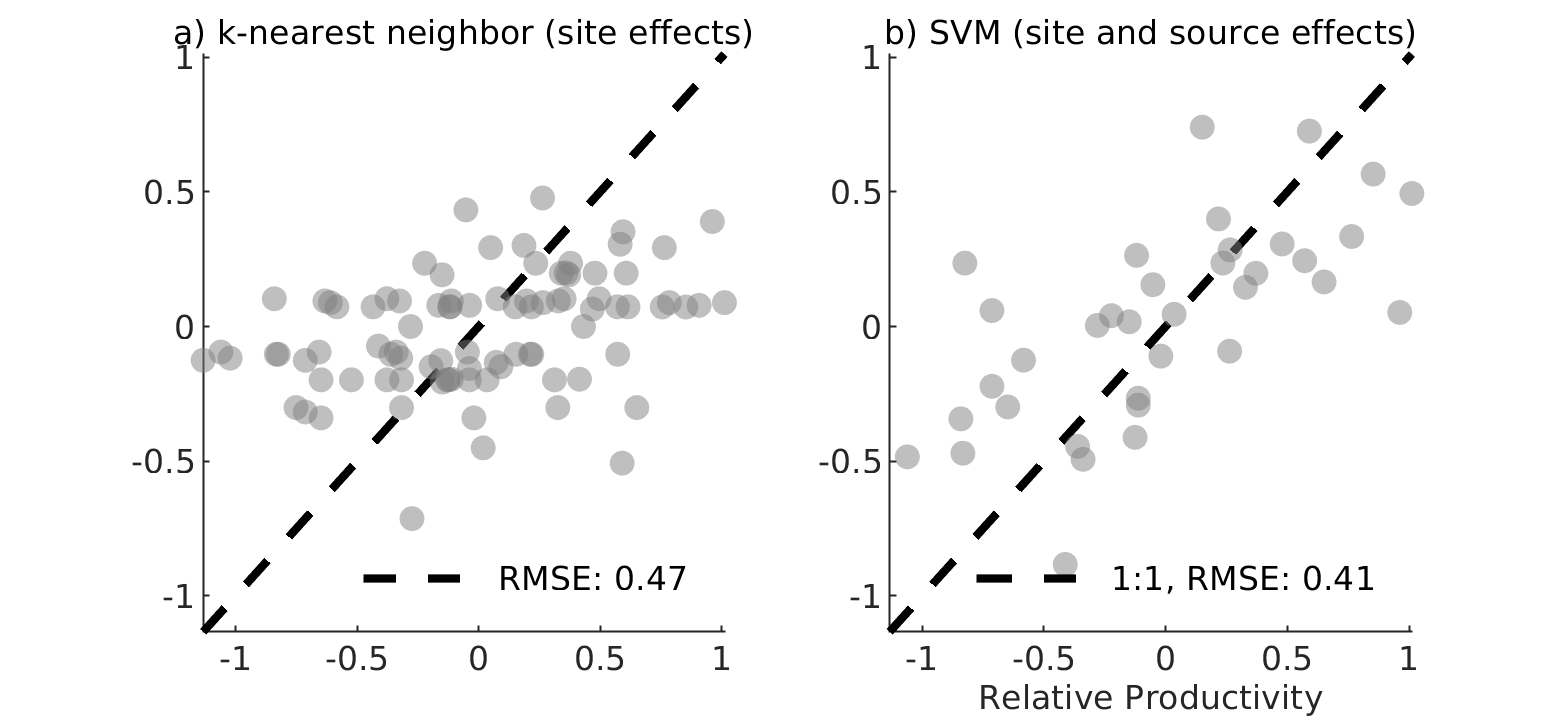
\includegraphics{figures/response_mw5.png}
\caption{Response plots (prediction versus observation) for the k-nearest neighbor algorithm and SVM models for $M_W$>5. Each point is an individual earthquake sequence. A perfect prediction would place all values on the 1:1 line. The SVM model outperforms the k-nearest neighbor model. Hold-one-out cross-validation ensures that the data for model calibration is separate from the prediction data. Combining both contextual information about the setting (crustal age) and the source (dip and normalized area) yields a root mean square value of 0.39. Particularly, the SVM model better predicts extreme cases (highly productive or unproductive).}
\label{fig:response}
\end{figure}

\begin{figure}
\centering
\label{fig:caltech}
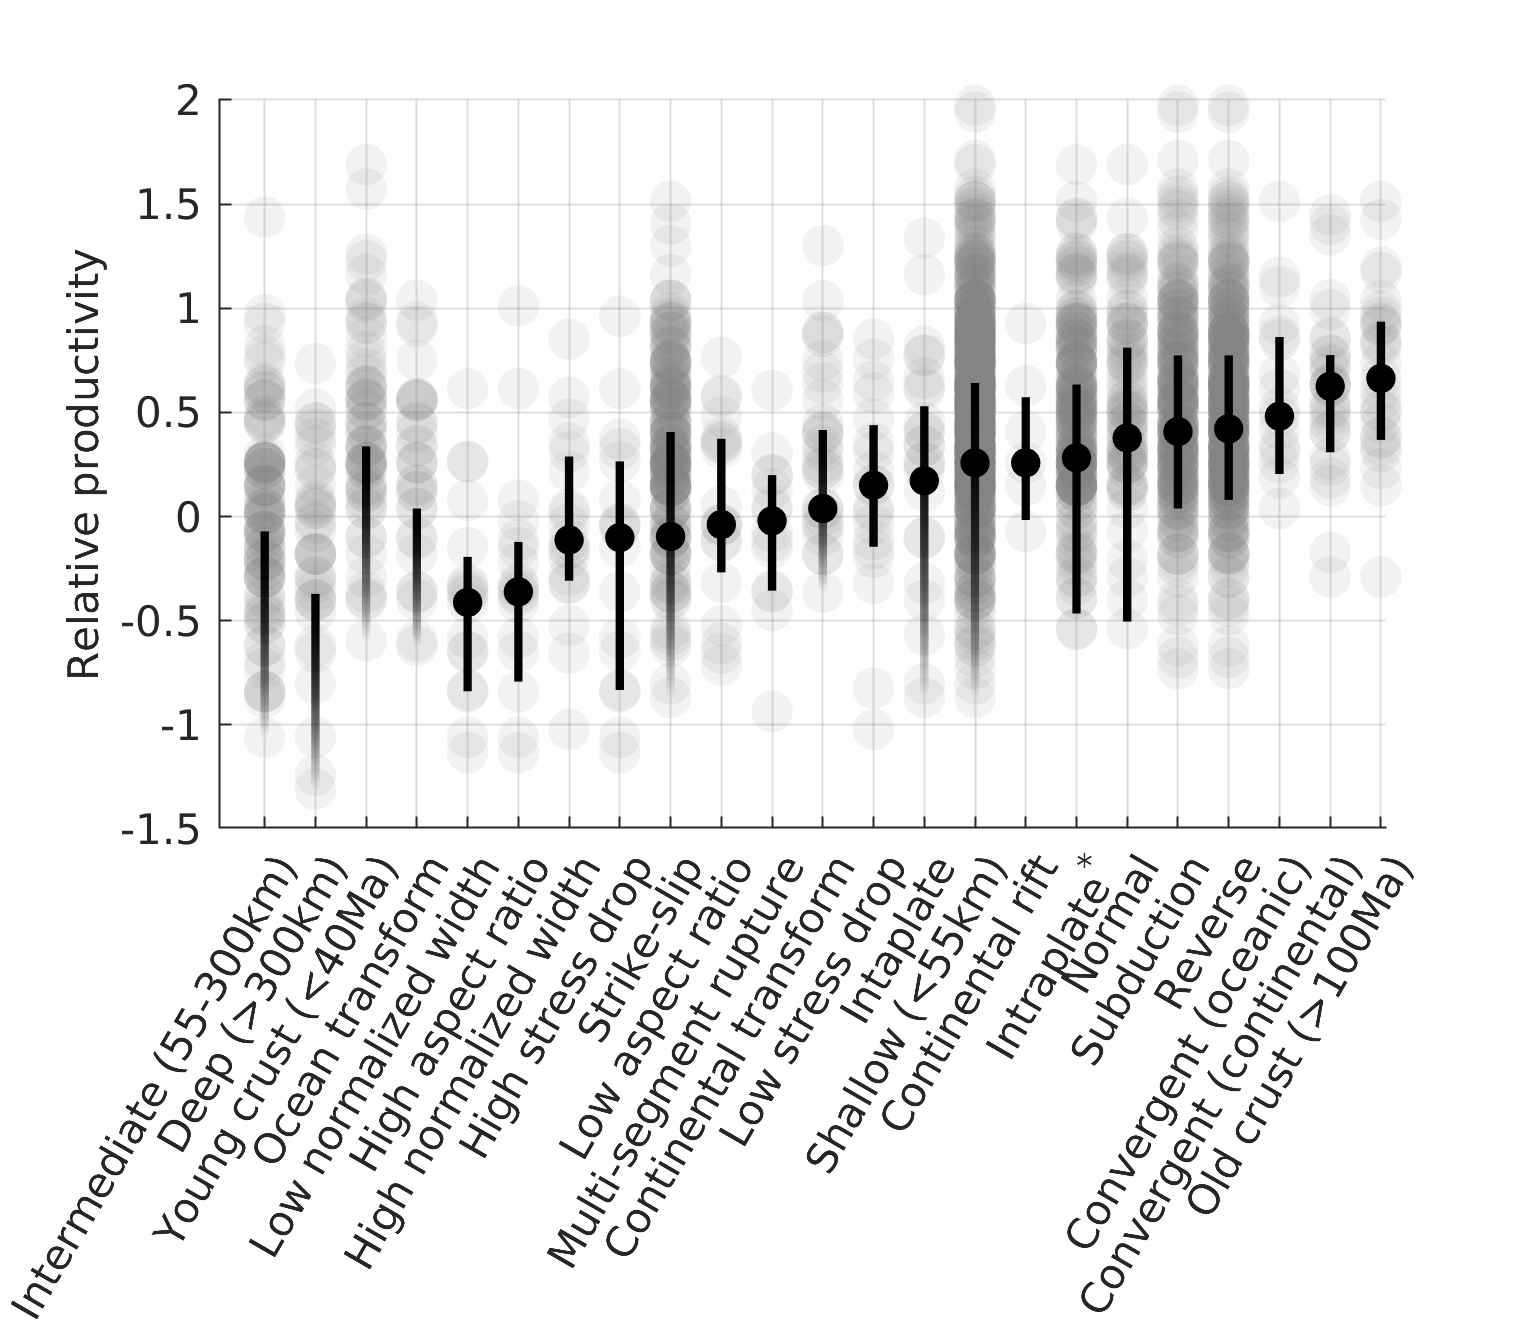
\includegraphics{figures/cal_tech_mw5.png}
\caption{Synthesis of relative productivity according to catalog subsets for $M_W$>5. The group considered here are the short list which best distinguished relative productivity based on our different lines of investigation. `High' and `low' subsets respectively refer to $>80$th and $<20$th percentile ranges of the data. Grey circles are individual mainshocks. Black points and error bars respectively indicate the median and interaquartile range of the subset. Fading error bars imply that mainshock sequences with no aftershocks are within the interquartile range of the data.}
\end{figure}   

%%%%%%%%%%%%%%%%%%%%%%%%%%%%%%%%%%%%%%%%%%%%%%%%%%%%%%%%%%%%%%%%%%%%%%%%    
    
\section*{Relative productivity as a function of miscellaneous parameters}

We present how the relative productivity changes as a function of each variable we tested for in this study. We show our results in Figure S\ref{fig:misc}.

\begin{figure}
\centering
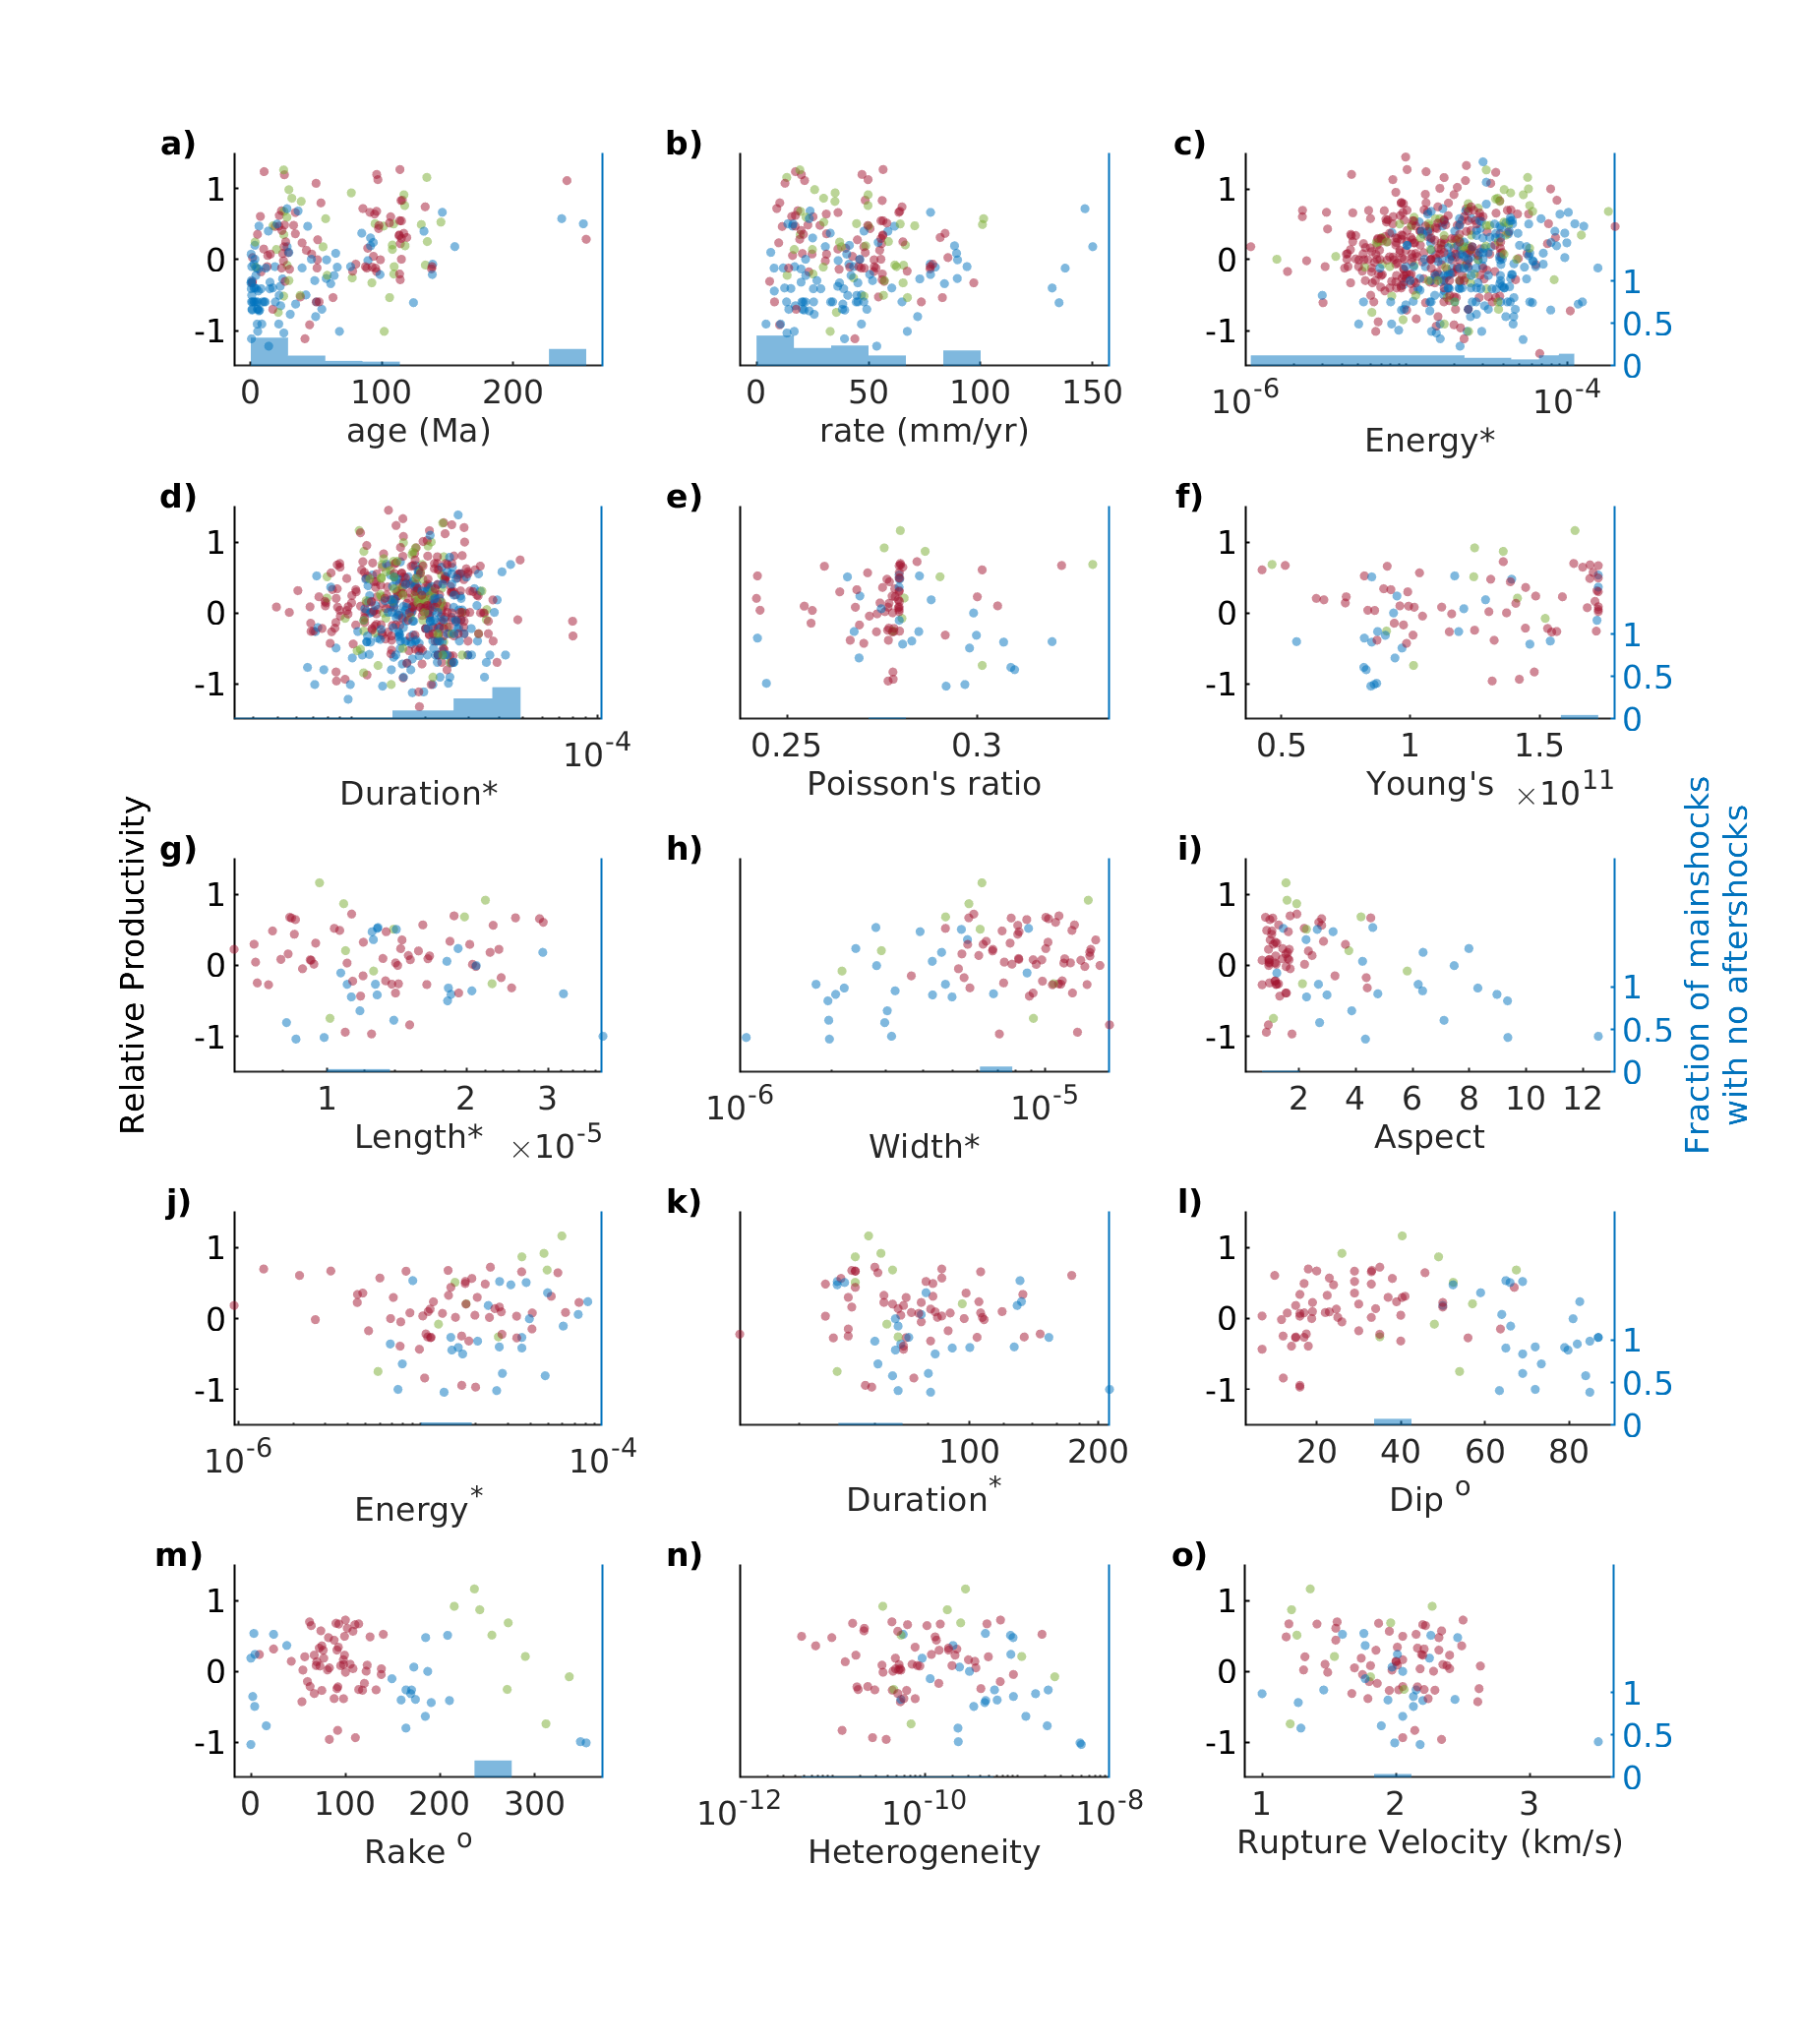
\includegraphics{figures/misc.png}
\caption{Miscellaneous setting and source attributes as a function of relative productivity ($N^*$). Source attributes that scale with magnitude are normalized (norm.) to eliminate any such dependence. Note that for the normalized rupture durations and the normalized radiated energy, we show their relationship to relative productivity for both the \citet{Convers2011GlobalMid2010} and \citet{Hayes2017} estimates. Mainshocks are color-coded by focal mechanism (strike-slip: blue, normal: green, and reverse: red). Note that a linear relationship has its limitations for more non-linear relationships (e.g. dip and rake).}
\label{fig:misc}
\end{figure}   

\section*{Catalogued Source Parameters}

We provide separately a table (Table S1) in .csv file format for all the source attributes we consider. The table includes earthquake date, latitude, longitude, depth, moment magnitude, moment, dip, rake, rupture velocity and duration as reported by \citet{Hayes2017}. We also include the focal mechanism, width, length, aspect ratio, slip heterogeneity and stress drop that we derived.

\bibliography{references.bib}

\end{document}